\chapter{Megvalósítás}

Ez a fejezet az alkalmazás konkrét implementációját mutatja be, a konfigurációtól az egyes rétegek megvalósításán át a legösszetettebb üzleti logikáig. Minden alfejezetben a tényleges forráskódon keresztül szemléltetjük az adott komponens működését.

% ============================================================
%  4.1  Az alkalmazás indítása és konfiguráció
% ============================================================
\section{Az alkalmazás indítása és konfiguráció}

\subsection{A belépési pont}

A Spring Boot alkalmazás belépési pontja az \texttt{ElearningApplication} osztály, amelyet a \texttt{@SpringBootApplication} annotáció jelöl. Ez az összetett annotáció három szerepet tölt be egyszerre: engedélyezi az automatikus komponensfelderítést (\texttt{@ComponentScan}), aktiválja az auto-configuration mechanizmust (\texttt{@EnableAutoConfiguration}), és maga is konfigurációs osztályként viselkedik (\texttt{@Configuration}).

\begin{java}[caption={Az alkalmazás belépési pontja},label=java:mainclass]
@SpringBootApplication
public class ElearningApplication {
    public static void main(String[] args) {
        SpringApplication.run(ElearningApplication.class, args);
    }
}
\end{java}

A \texttt{SpringApplication.run()} hívás indítja el a beágyazott Tomcat szervert, inicializálja az IoC konténert és futtatja az összes \texttt{CommandLineRunner} implementációt — köztük az adatinicializálót.

\subsection{Maven függőségek}

A projekt építési leírója a \texttt{pom.xml} fájl, amelynek szülőprojektje a \texttt{spring-boot-starter-parent} 3.5.6-os verziója. Ez a szülőprojekt egységesen kezeli az összes Spring-függőség verzióját. A főbb függőségek:

\begin{itemize}
    \item \texttt{spring-boot-starter-web} – beágyazott Tomcat és Spring MVC;
    \item \texttt{spring-boot-starter-data-jpa} – Spring Data JPA és Hibernate ORM;
    \item \texttt{spring-boot-starter-security} – Spring Security szűrőlánc;
    \item \texttt{spring-boot-starter-validation} – Bean Validation (Jakarta Validation API);
    \item \texttt{spring-boot-starter-thymeleaf} – Thymeleaf sablon-motor;
    \item \texttt{spring-boot-starter-mail} – JavaMail integráció SMTP-küldéshez;
    \item \texttt{thymeleaf-extras-springsecurity6} – \texttt{sec:authorize} névtér a sablonokban;
    \item \texttt{h2} (runtime scope) – beágyazott H2 memória-adatbázis fejlesztési célra;
    \item \texttt{poi-ooxml} és \texttt{poi-scratchpad} 5.2.5 – Apache POI \texttt{.pptx} és \texttt{.ppt} feldolgozáshoz;
    \item \texttt{pdfbox} 2.0.30 – Apache PDFBox PDF-generáláshoz (explicit verziószám szükséges, mert a Spring Boot szülőprojekt nem kezeli);
    \item \texttt{spring-security-test} (test scope) – \texttt{@WithMockUser} és CSRF-szimulációs segédeszközök teszteléshez.
\end{itemize}

\subsection{Az \texttt{application.properties} konfiguráció}

A legfontosabb konfigurációs beállítások:

\begin{itemize}
    \item \texttt{spring.datasource.url=jdbc:h2:mem:testdb} – H2 memória-adatbázis;
    \item \texttt{spring.jpa.hibernate.ddl-auto=create-drop} – séma létrehozása indításkor, törlése leálláskor;
    \item \texttt{spring.servlet.multipart.max-file-size=50MB} – fájlfeltöltési méretkorlát;
    \item \texttt{spring.mail.host}, \texttt{port}, \texttt{username}, \texttt{password} – Gmail SMTP konfiguráció;
    \item \texttt{app.mail.from} és \texttt{app.base-url} – egyedi property-k az \texttt{EmailService} számára;
    \item \texttt{h2.console.security.enabled=false} – H2 konzol letiltása.
\end{itemize}

% ============================================================
%  4.2  A forráskód szerkezete
% ============================================================
\section{A forráskód szerkezete}

A Java forráskód az \texttt{src/main/java/com/melearning/elearning/} főcsomagban helyezkedik el, öt alcsomag szerint rendezve:

\begin{itemize}
    \item \texttt{config/} – \texttt{SecurityConfig} és \texttt{DataInitializer};
    \item \texttt{controller/} – \texttt{AuthController}, \texttt{CourseController}, \texttt{DashboardController}, \texttt{HomeController}, \texttt{LessonController}, \texttt{PresentationController}, \texttt{QuizController}, \texttt{UserController};
    \item \texttt{model/} – \texttt{User}, \texttt{Course}, \texttt{Lesson}, \texttt{Presentation}, \texttt{Quiz}, \texttt{Question}, \texttt{QuizResult}, \texttt{Role};
    \item \texttt{repository/} – \texttt{CourseRepository}, \texttt{LessonRepository}, \texttt{PresentationRepository}, \texttt{QuestionRepository}, \texttt{QuizRepository}, \texttt{QuizResultRepository}, \texttt{UserRepository};
    \item \texttt{service/} – \texttt{CourseService}, \texttt{CustomUserDetailsService}, \texttt{EmailService}, \texttt{LessonService}, \texttt{PresentationService}, \texttt{QuizService}, \texttt{UserService}.
\end{itemize}

A csomagok közötti függőségek egyirányúak: controller $\to$ service $\to$ repository $\to$ model. 

% ============================================================
%  4.3  Adatmodell megvalósítása
% ============================================================
\section{Adatmodell megvalósítása}

\subsection{A User entitás}

A \texttt{User} osztályt a \texttt{@Table(name = "users")} annotáció jelöli, mert a \texttt{USER} szó fenntartott kulcsszó a H2 SQL dialektusában. Az egyediségi megszorítások adatbázis szinten garantálják, hogy két felhasználó ne regisztrálhasson azonos felhasználónévvel vagy e-mail-címmel.

\begin{java}[caption={A User entitás főbb mezői},label=java:userentity]
@Entity
@Table(name = "users")
public class User {

    @Id
    @GeneratedValue(strategy = GenerationType.IDENTITY)
    private Long id;

    @NotBlank @Size(max = 50)
    @Column(unique = true)
    private String username;

    @NotBlank @Size(max = 100) @Email
    @Column(unique = true)
    private String email;

    @NotBlank @Size(max = 100)
    private String password;

    @Enumerated(EnumType.STRING)
    private Role role;

    private LocalDateTime createdAt;

    @ManyToMany(mappedBy = "enrolledUsers")
    private Set<Course> enrolledCourses = new HashSet<>();

    public User() { this.createdAt = LocalDateTime.now(); }
    // ... getterek, setterek
}
\end{java}

A \texttt{@Enumerated(EnumType.STRING)} gondoskodik arról, hogy a \texttt{Role} enum értéke szövegként kerüljön az adatbázisba, megvédve az adatokat az enum-sorrend jövőbeli megváltozásától.

\subsection{A Course entitás}

A \texttt{Course} entitás a rendszer központi eleme, amely \texttt{Lesson}, \texttt{Quiz} és beiratkozott \texttt{User} entitásokkal is kapcsolatban áll.

\begin{java}[caption={A Course entitás kapcsolatai},label=java:courseentity]
@Entity
@Table(name = "courses")
public class Course {

    @ManyToOne
    @JoinColumn(name = "instructor_id")
    private User instructor;

    @OneToMany(mappedBy = "course",
               cascade = CascadeType.ALL, orphanRemoval = true)
    private List<Lesson> lessons = new ArrayList<>();

    @OneToMany(mappedBy = "course",
               cascade = CascadeType.ALL, orphanRemoval = true)
    private List<Quiz> quizzes = new ArrayList<>();

    @ManyToMany
    @JoinTable(
        name = "course_enrollments",
        joinColumns = @JoinColumn(name = "course_id"),
        inverseJoinColumns = @JoinColumn(name = "user_id")
    )
    private Set<User> enrolledUsers = new HashSet<>();
    // ...
}
\end{java}

A \texttt{CascadeType.ALL} és \texttt{orphanRemoval = true} kombináció a \texttt{Lesson} és \texttt{Quiz} kapcsolatoknál biztosítja, hogy kurzustörléskor az összes hozzá tartozó lecke és kvíz automatikusan törlődjön.

\subsection{A Lesson entitás}

A \texttt{Lesson} entitás egy kurzuson belüli tematikus egységet képvisel. Tartalmaz egy szöveges tartalommezőt (\texttt{@Column(columnDefinition = "TEXT")}), egy sorrendi indexet a leckék rendezéséhez, és egy közvetlen kapcsolatot a hozzá csatolt prezentációkhoz.

\begin{java}[caption={A Lesson entitás felépítése},label=java:lessonentity]
@Entity
@Table(name = "lessons")
public class Lesson {

    @Id
    @GeneratedValue(strategy = GenerationType.IDENTITY)
    private Long id;

    @NotBlank @Size(max = 100)
    private String title;

    @Column(columnDefinition = "TEXT")
    private String content;

    private Integer orderIndex;

    @ManyToOne
    @JoinColumn(name = "course_id")
    private Course course;

    @OneToMany(mappedBy = "lesson", cascade = CascadeType.ALL)
    private List<Presentation> presentations = new ArrayList<>();

    private LocalDateTime createdAt;

    public Lesson() { this.createdAt = LocalDateTime.now(); }
    // ...
}
\end{java}

A leckék sorrendbe rendezése az \texttt{orderIndex} mező alapján történik, amelyet a \texttt{LessonRepository} a \texttt{findByCourseIdOrderByOrderIndexAsc()} metódussal vesz figyelembe. A \texttt{presentations} lista lehetővé teszi, hogy minden leckéhez közvetlenül csatoljunk feltöltött anyagokat, így a hallgatók a kurzus megtekintésekor lecke-szinten is böngészhetnek a prezentációk között.

\subsection{A Presentation entitás}

Az optimalizálás során a \texttt{Presentation} entitás két kapcsolattal rendelkezik: a kötelező \texttt{Course}-kapcsolat mellett egy opcionális \texttt{Lesson}-kapcsolat is bekerült, \texttt{FetchType.LAZY} betöltési stratégiával.

\begin{java}[caption={A Presentation entitás bővített kapcsolatai},label=java:presentationentity]
@Entity
@Table(name = "presentations")
public class Presentation {

    @Lob
    @Column(columnDefinition = "LONGBLOB")
    private byte[] fileData;

    @ManyToOne
    @JoinColumn(name = "course_id")
    private Course course;

    @ManyToOne(fetch = FetchType.LAZY)
    @JoinColumn(name = "lesson_id")
    private Lesson lesson;

    private Integer orderIndex;
    // ...
}
\end{java}

A \texttt{lesson} mező \texttt{null} értékű lehet: ez olyan prezentációknak felel meg, amelyeket az oktató kurzusszinten töltött fel, nem konkrét leckéhez rendelve. A \texttt{FetchType.LAZY} beállítás megakadályozza, hogy a prezentáció listázásakor szükségtelenül betöltődjön a kapcsolódó lecke teljes objektuma.

\subsection{A Quiz és Question entitás}

A \texttt{Quiz} osztályban az osztályzatot számító \texttt{calculateGrade(int percentage)} metódus az entitásban helyezkedik el, mert az osztályzatszámítás szorosan kötődik a kvíz egyedi ponthatáraihoz.

\begin{java}[caption={A Quiz entitás pontszámítási metódusa},label=java:quizgrade]
@Entity
@Table(name = "quizzes")
public class Quiz {

    private Integer excellentThreshold = 85;
    private Integer goodThreshold      = 70;
    private Integer averageThreshold   = 55;
    private Integer passingThreshold   = 40;
    private Boolean allowMultipleAttempts = true;

    @OneToMany(mappedBy = "quiz",
               cascade = CascadeType.ALL,
               orphanRemoval = true,
               fetch = FetchType.EAGER)
    private List<Question> questions = new ArrayList<>();

    public int calculateGrade(int percentage) {
        if (percentage >= excellentThreshold) return 5;
        if (percentage >= goodThreshold)      return 4;
        if (percentage >= averageThreshold)   return 3;
        if (percentage >= passingThreshold)   return 2;
        return 1;
    }
    // ...
}
\end{java}

A kérdések kapcsolatánál \texttt{FetchType.EAGER} lett beállítva, mert a kvíz megjelenítésekor mindig szükség van az összes kérdésre. A \texttt{Question} entitás négy fix válaszlehetőséget (\texttt{optionA}–\texttt{optionD}) tárol külön mezőkben, a helyes választ pedig egy betűjeles \texttt{correctOption} mező jelöli.

\subsection{A QuizResult entitás}

A \texttt{QuizResult} a \texttt{percentage} és \texttt{grade} mezőket tárolt értékekként rögzíti, ami lehetővé teszi az összesített statisztikák hatékony számítását és a visszamenőleges osztályzat-újraszámítást a ponthatárok módosításakor.

% ============================================================
%  4.4  Adatinicializálás
% ============================================================
\section{Adatinicializálás}

A \texttt{DataInitializer} osztály a \texttt{CommandLineRunner} interfészt implementálja; \texttt{run()} metódusát a Spring Boot az alkalmazáskontextus teljes inicializálása után automatikusan meghívja. Az \texttt{if (userRepository.count() == 0)} feltétel biztosítja, hogy az inicializálás csak üres adatbázis esetén fusson le.

\begin{java}[caption={Adatinicializáló — tesztfelhasználók létrehozása},label=java:datainit]
@Component
public class DataInitializer implements CommandLineRunner {

    @Autowired private UserRepository   userRepository;
    @Autowired private LessonRepository lessonRepository;
    @Autowired private PasswordEncoder  passwordEncoder;

    @Override
    public void run(String... args) throws Exception {
        if (userRepository.count() == 0) {
            initializeUsers();
        }
    }

    private void initializeUsers() {
        User admin = new User();
        admin.setUsername("admin");
        admin.setEmail("admin@elearning.hu");
        admin.setPassword(passwordEncoder.encode("admin123"));
        admin.setRole(Role.ADMIN);
        userRepository.save(admin);

        User instructor = new User();
        instructor.setUsername("instructor");
        instructor.setEmail("instructor@elearning.hu");
        instructor.setPassword(passwordEncoder.encode("instructor123"));
        instructor.setRole(Role.INSTRUCTOR);
        userRepository.save(instructor);
    }

    private void createLesson(Course course, String title,
                               String content, int order) {
        Lesson lesson = new Lesson();
        lesson.setTitle(title);
        lesson.setContent(content);
        lesson.setOrderIndex(order);
        lesson.setCourse(course);
        lessonRepository.save(lesson);
    }
}
\end{java}

Az osztály elsődleges célja a tesztkörnyezet gyors felállítása, biztosítva a fejlesztéshez szükséges alapértelmezett tesztadatok (mock adatok) automatikus betöltését.

% ============================================================
%  4.5  Biztonsági konfiguráció
% ============================================================
\section{Biztonsági konfiguráció}

\subsection{A SecurityConfig osztály}
A \texttt{SecurityConfig} osztály az alkalmazás biztonsági infrastruktúrájának központi eleme. Feladata a hitelesítés és a jogosultságkezelés szabályozása, amelyet három alapvető Bean definiálásával valósít meg:

\begin{itemize}
\item \textbf{PasswordEncoder}: A jelszavak biztonságos, BCrypt algoritmussal történő hash-eléséért felel.
\item \textbf{AuthenticationManager}: A felhasználók azonosításának folyamatát koordinálja.
\item \textbf{SecurityFilterChain}: Meghatározza a védelmi szűrőket, valamint az URL-alapú hozzáférési szabályokat.
\end{itemize}

\begin{java}[caption={A SecurityFilterChain konfigurálása},label=java:securityconfig]
@Bean
public SecurityFilterChain filterChain(HttpSecurity http)
        throws Exception {

    http.userDetailsService(userDetailsService);

    http.authorizeHttpRequests(authz -> {
        if (h2ConsoleEnabled) {
            authz.requestMatchers("/h2-console/**").hasRole("ADMIN");
        }

        authz.requestMatchers(
                "/", "/login", "/register", "/about",
                "/css/**", "/js/**", "/images/**"
        ).permitAll();

        authz.requestMatchers(
                "/courses/create",
                "/courses/*/manage",
                "/courses/*/delete",
                "/courses/*/delete-presentation",
                "/courses/*/add-student",
                "/courses/*/remove-student",
                "/courses/*/add-presentations",
                "/courses/*/quizzes/create",
                "/courses/*/quizzes/*/delete",
                "/courses/*/quizzes/*/thresholds",
                "/courses/*/quizzes/*/results"
        ).hasAnyRole("INSTRUCTOR", "ADMIN");

        authz.requestMatchers(
                "/dashboard/admin/**"
        ).hasRole("ADMIN");

        authz.anyRequest().authenticated();
    });

    http.formLogin(form -> form
            .loginPage("/login")
            .defaultSuccessUrl("/", true)
            .failureUrl("/login?error=true")
            .permitAll()
    );

    http.logout(logout -> logout
            .logoutSuccessUrl("/")
            .permitAll()
    );

    if (h2ConsoleEnabled) {
        http.csrf(csrf -> csrf
                .ignoringRequestMatchers("/h2-console/**"));
        http.headers(headers -> headers
                .frameOptions(frame -> frame.sameOrigin()));
    }

    return http.build();
}
\end{java}

A biztonsági szabályrendszer az alábbi hozzáférési szinteket különíti el:
\begin{enumerate}
\item \textbf{Nyilvános elérés:} A kezdőoldal, a regisztráció, a statikus erőforrások (CSS, JS), valamint az \texttt{/about} tájékoztató oldal bárki számára elérhető.
\item \textbf{Oktatói és Admin jogosultság:} A kurzusok kezeléséhez, törléséhez és a kvízek adminisztrációjához szükséges funkciók az \texttt{INSTRUCTOR} vagy \texttt{ADMIN} szerepkörrel rendelkező felhasználókra korlátozódnak.
\item \textbf{Kizárólagos Admin elérés:} A rendszerszintű beállítások, a felhasználói fiókok kezelése és — engedélyezés esetén — a H2-konzol elérése csak az \texttt{ADMIN} szerepkör számára megengedett.
\end{enumerate}

\subsection{A CustomUserDetailsService}

A \texttt{CustomUserDetailsService} implementálja a Spring Security \texttt{UserDetailsService} interfészét. A bejelentkezéskor a \texttt{loadUserByUsername()} metódus a \texttt{UserRepository}-n keresztül tölti be a felhasználót, és a \texttt{CustomUserPrincipal} belső osztályba csomagolja.

\begin{java}[caption={CustomUserDetailsService és CustomUserPrincipal},label=java:userdetails]
@Service
public class CustomUserDetailsService implements UserDetailsService {

    @Autowired
    private UserRepository userRepository;

    @Override
    public UserDetails loadUserByUsername(String username)
            throws UsernameNotFoundException {
        User user = userRepository.findByUsername(username)
                .orElseThrow(() -> new UsernameNotFoundException(
                        "Felhasználó nem található: " + username));
        return new CustomUserPrincipal(user);
    }

    public static class CustomUserPrincipal implements UserDetails {
        private final User user;

        public CustomUserPrincipal(User user) { this.user = user; }

        @Override
        public Collection<? extends GrantedAuthority> getAuthorities() {
            return Collections.singleton(new SimpleGrantedAuthority(
                    "ROLE_" + user.getRole().name()));
        }

        @Override public String getPassword() { return user.getPassword(); }
        @Override public String getUsername() { return user.getUsername(); }
        @Override public boolean isAccountNonExpired()     { return true; }
        @Override public boolean isAccountNonLocked()      { return true; }
        @Override public boolean isCredentialsNonExpired() { return true; }
        @Override public boolean isEnabled()               { return true; }

        public User getUser() { return user; }
    }
}
\end{java}

A \texttt{getUser()} segédmetódus lehetővé teszi, hogy a kontrollerekben az \texttt{Authentication} objektumból közvetlenül elérjük a \texttt{User} entitást anélkül, hogy külön adatbázis-lekérdezést kellene indítani.

% ============================================================
%  4.6  Adatelérési réteg
% ============================================================
\section{Adatelérési réteg}

A Spring Data JPA repository interfészek az \texttt{JpaRepository<T, ID>} alaptípust terjesztik ki, az egyedi lekérdezéseket pedig metódusnév-alapú query derivation segítségével valósítják meg.

\begin{java}[caption={A CourseRepository és a LessonRepository},label=java:repos]
@Repository
public interface CourseRepository extends JpaRepository<Course, Long> {
    List<Course> findByInstructor(User instructor);
    List<Course> findByEnrolledUsersContaining(User user);
    List<Course> findByIsPublicTrue();
}

@Repository
public interface LessonRepository extends JpaRepository<Lesson, Long> {
    List<Lesson> findByCourseIdOrderByOrderIndexAsc(Long courseId);
}
\end{java}

A \texttt{LessonRepository} egyetlen egyedi metódusa rendezett lekérdezést végez: a \texttt{findByCourseIdOrderByOrderIndexAsc()} az \texttt{orderIndex} mező szerint növekvő sorrendben adja vissza a leckéket, ezért nincs szükség Java-oldalon utólagos rendezésre.

\begin{java}[caption={A QuizResultRepository egyedi metódusai},label=java:quizresultrepo]
@Repository
public interface QuizResultRepository
        extends JpaRepository<QuizResult, Long> {

    List<QuizResult> findByUser(User user);
    List<QuizResult> findByQuiz(Quiz quiz);
    boolean existsByUserAndQuiz(User user, Quiz quiz);
    Optional<QuizResult> findTopByUserAndQuizOrderByCompletedAtDesc(
            User user, Quiz quiz);
}
\end{java}

A \texttt{findTopByUserAndQuizOrderByCompletedAtDesc} a megadott felhasználóhoz és kvízhez tartozó legfrissebb eredményt adja vissza egyetlen rekordként, amelyet az egyszeri kitöltési logika használ az előző eredmény megjelenítéséhez.

% ============================================================
%  4.7  Szolgáltatási réteg
% ============================================================
\section{Szolgáltatási réteg}

\subsection{UserService}

A \texttt{UserService} az összes felhasználóhoz kapcsolódó üzleti logikát összefogja: regisztrációt, profilkezelést, jelszóváltoztatást és törlést egyaránt.
A \texttt{saveUser()} az új felhasználók regisztrációjakor használatos: a jelszót BCrypt-tel enkódolja mentés előtt. A profilszerkesztési végpontok az \texttt{updateUser()} metódust hívják meg.
A felhasználó jelszavának megváltoztatása a \texttt{changePassword()} metóduson keresztül történik, amely először ellenőrzi, hogy a megadott jelenlegi jelszó egyezik-e a tárolt hash-sel. Sikeres ellenőrzés után enkódolja és menti az új jelszót, majd az \texttt{EmailService}-en keresztül biztonsági értesítőt küld.

\begin{java}[caption={Jelszóváltoztatás logikája a UserService-ben},label=java:userservice_pw]
public boolean changePassword(User user,
        String currentPassword,
        String newPassword) {
    if (!passwordEncoder.matches(currentPassword, user.getPassword())) {
        return false;
    }
    user.setPassword(passwordEncoder.encode(newPassword));
    userRepository.save(user);
    emailService.sendPasswordChangeEmail(
            user.getEmail(), user.getFirstName());
    return true;
}
\end{java}

A \texttt{UserController} a profiloldalt két elkülönített \texttt{POST} végponton kezeli, amelyek a felhasználó saját adatait módosítják:

\begin{itemize}
\item \textbf{\texttt{POST /profile/update-email}} — e-mail-cím módosítása. Foglaltság-ellenőrzés után menti az új e-mail-címet, és értesítő e-mailt küld az új címre. Ez a művelet nem igényel újrabelépést.
\item \textbf{\texttt{POST /profile/update-password}} — jelszó módosítása. Három feltételt ellenőriz egymás után: a jelenlegi jelszó helyességét (\texttt{passwordEncoder.matches()}), az új jelszó és a megerősítés egyezőségét, valamint a minimális jelszóhosszt (6 karakter). Sikeres módosítás esetén a munkamenet érvénytelenítésre kerül (\texttt{Security\-Context\-Holder.\-clear\-Context()},\linebreak[0] \texttt{request.\-getSession().\-invalidate()}), és a felhasználónak az új jelszóval kell újra bejelentkeznie — enélkül a Spring Security a lejárt munkamenetben szereplő régi hitelesítési adatokkal operálna tovább.
\end{itemize}

\subsection{CourseService}

A \texttt{CourseService} osztály a kurzusokhoz kapcsolódó üzleti logikát fogja össze. Metódusai lefedik a kurzusok teljes életciklusát: létrehozást, módosítást és törlést, valamint a különböző szempontú lekérdezéseket — oktató szerinti szűrést, nyilvános kurzusok listázását és beiratkozott hallgatók alapján való keresést. A beiratkozás kezelése szintén itt történik: a \texttt{enrollUser()} és \texttt{unenrollUser()} metódusok gondoskodnak a \texttt{course\_enrollments} kapcsolótábla karbantartásáról. A kurzustörlés \texttt{@Transactional} annotációval védett, és a törlés előtt eltávolítja a kapcsolódó prezentációkat, hogy idegen kulcs megsértése ne okozzon adatbázis-hibát.

\begin{java}[caption={Kurzustörlés — Presentation előzetes törlésével},label=java:deletecourse]
@Transactional
public void deleteCourse(Long id) {
    courseRepository.findById(id).ifPresent(course -> {
        presentationRepository.deleteByCourse(course);
    });
    courseRepository.deleteById(id);
}
\end{java}

A leckék és kvízek \texttt{CascadeType.ALL, orphanRemoval = true} beállításuk révén automatikusan törlődnek a kurzussal együtt.

\subsection{LessonService}

A \texttt{LessonService} a lecke életciklusának egyszerű kezelését biztosítja: mentést, kurzus-azonosító szerinti rendezett lekérdezést és ID alapú keresést.

\begin{java}[caption={A LessonService metódusai},label=java:lessonservice]
@Service
public class LessonService {

    @Autowired
    private LessonRepository lessonRepository;

    public Lesson save(Lesson lesson) {
        return lessonRepository.save(lesson);
    }

    public List<Lesson> findByCourseId(Long courseId) {
        return lessonRepository
                .findByCourseIdOrderByOrderIndexAsc(courseId);
    }

    public Optional<Lesson> findById(Long id) {
        return lessonRepository.findById(id);
    }
}
\end{java}

\subsection{QuizService}

A \texttt{QuizService.saveQuiz()} metódusa gondoskodik a kétirányú \texttt{Quiz}–\texttt{Question} JPA kapcsolat helyes beállításáról: minden kérdéshez explicit beállítja a szülő-kvíz referenciát, mert enélkül a \texttt{quiz\_id} idegenkulcs-mező \texttt{NULL} értékkel kerülne mentésre.

\begin{java}[caption={QuizService – kétirányú JPA kapcsolat kezelése mentésnél},label=java:quizservice]
public Quiz saveQuiz(Quiz quiz) {
    if (quiz.getQuestions() != null) {
        quiz.getQuestions().forEach(q -> q.setQuiz(quiz));
    }
    return quizRepository.save(quiz);
}
\end{java}

% ============================================================
%  4.8  Felhasználókezelés megvalósítása
% ============================================================
\section{Felhasználókezelés megvalósítása}

\subsection{Regisztráció és bejelentkezés}

Az \texttt{AuthController} kétszintű validációt alkalmaz regisztrációkor: Bean Validation ellenőrzi a mezők formátumát, az alkalmazás üzleti logikája pedig a felhasználónév és e-mail egyediségét.

\begin{figure}[h!]
    \centering
    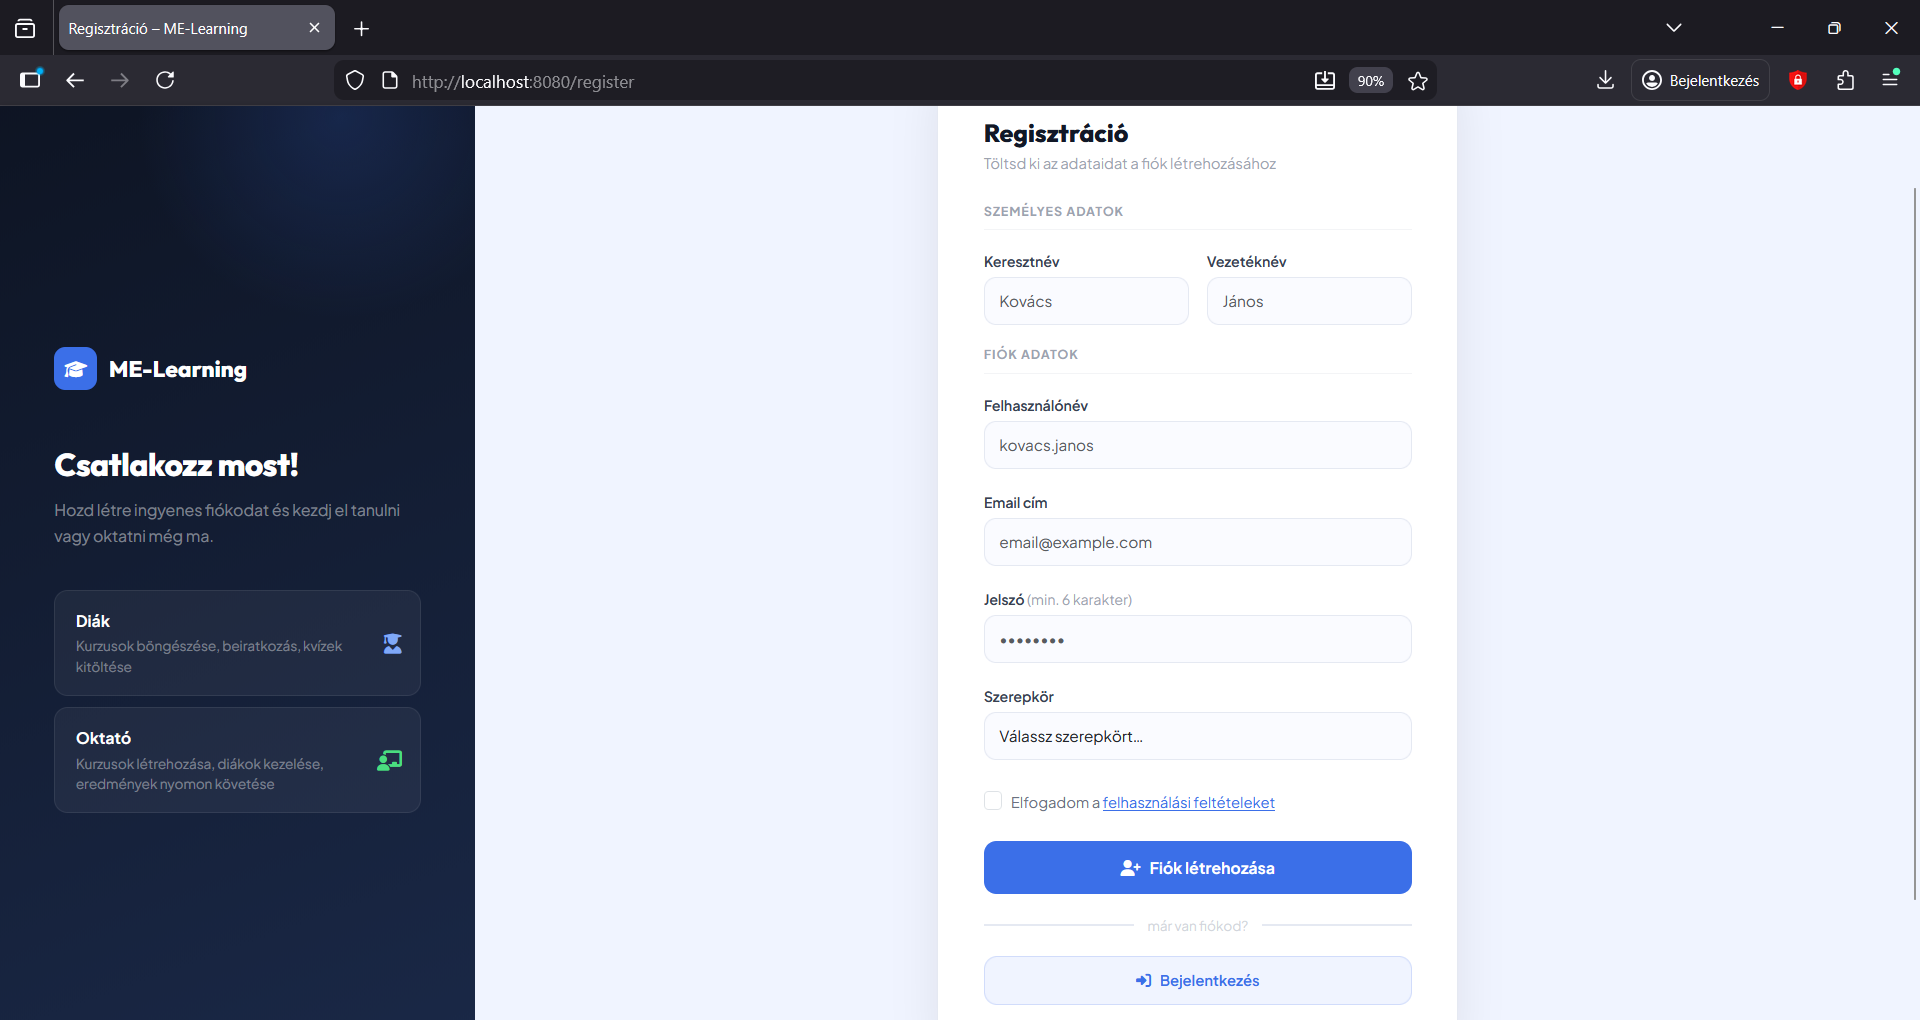
\includegraphics[width=1\textwidth]{images/Regisztracio.png}
    \caption{Regisztrációs oldal szemléltetése.}
    \label{fig:Regisztrációs_oldal}
\end{figure}

\begin{figure}[h!]
    \centering
    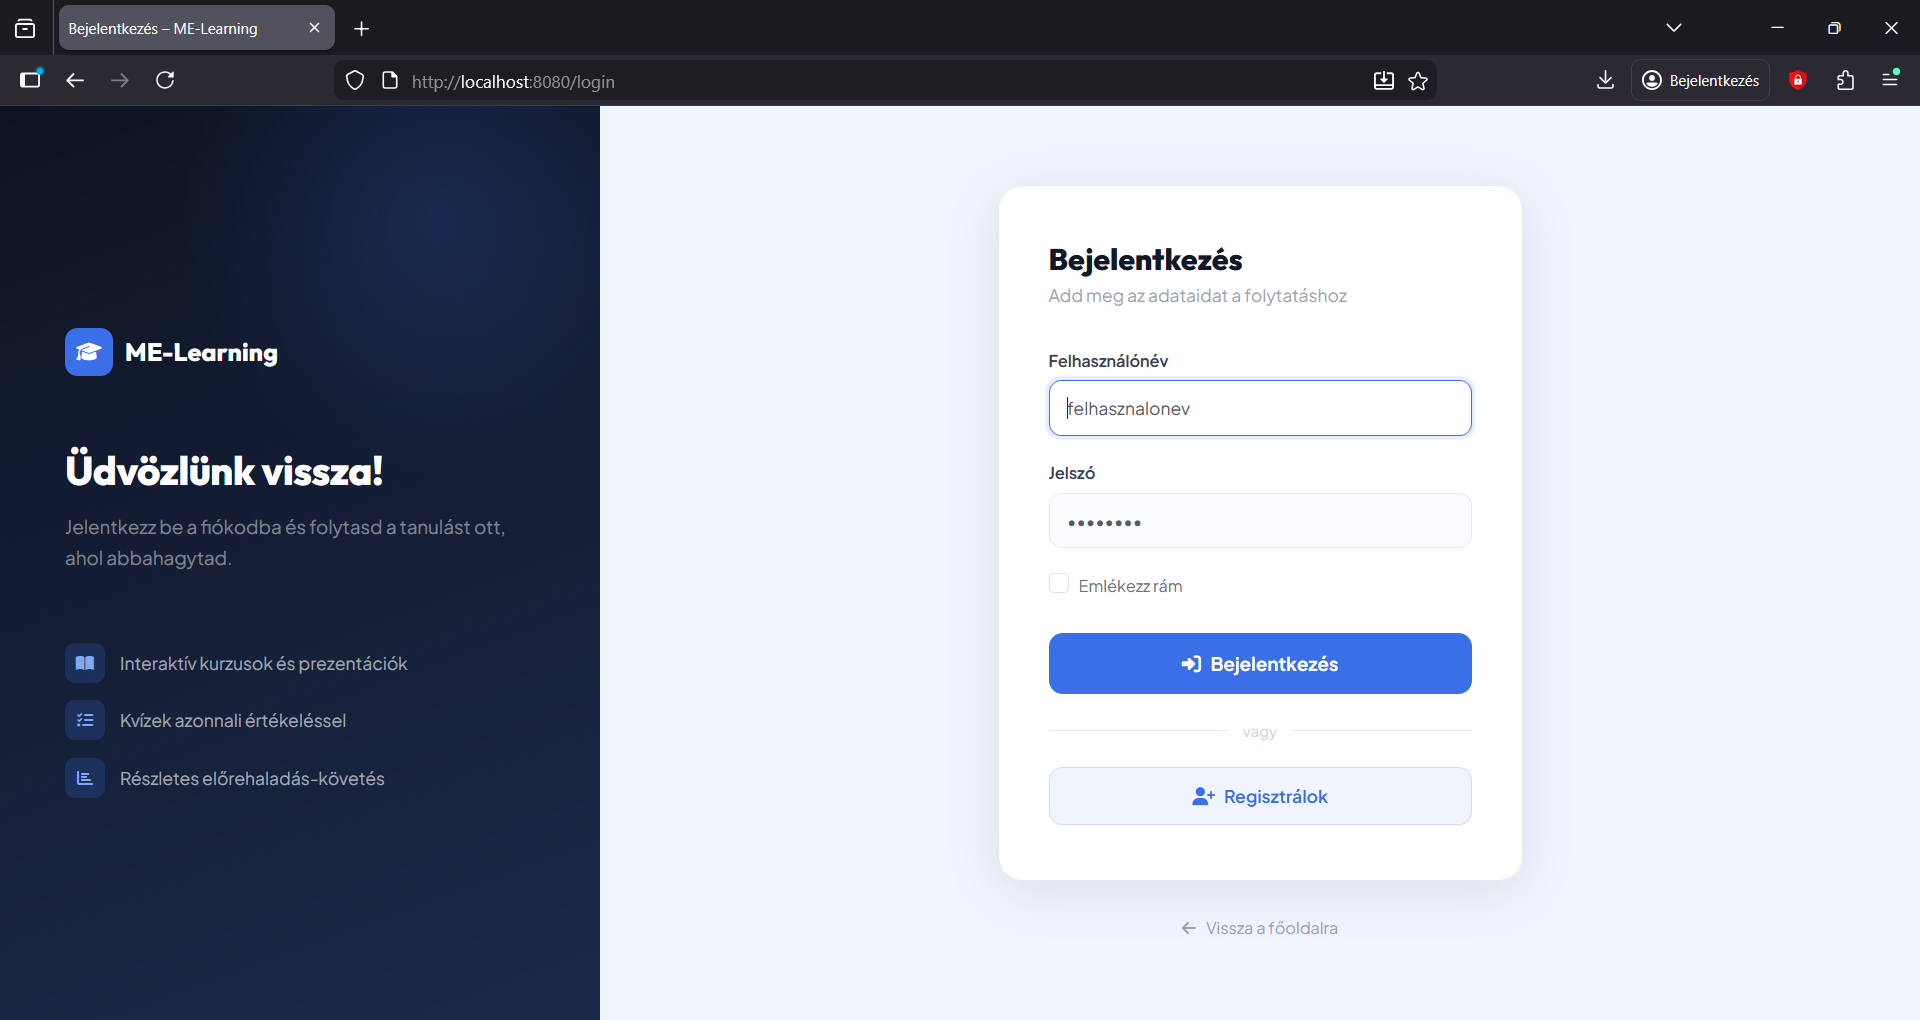
\includegraphics[width=1\textwidth]{images/Bejelentkezes.png}
    \caption{Bejelentkezési oldal szemléltetése.}
    \label{fig:Regisztrációs_oldal}
\end{figure}

\begin{java}[caption={Az AuthController regisztrációs POST végpontja},label=java:authcontroller]
@PostMapping("/register")
public String registerUser(
        @Valid @ModelAttribute("user") User user,
        BindingResult result, Model model,
        RedirectAttributes redirectAttributes) {

    if (result.hasErrors()) return "register";

    if (userService.existsByUsername(user.getUsername())) {
        model.addAttribute("error", "A felhasználónév már foglalt!");
        return "register";
    }
    if (userService.existsByEmail(user.getEmail())) {
        model.addAttribute("error",
                "Az email cím már használatban van!");
        return "register";
    }

    try {
        userService.saveUser(user);
        emailService.sendRegistrationEmail(
                user.getEmail(), user.getFirstName());
        redirectAttributes.addFlashAttribute("success",
                "Sikeres regisztráció! Most már bejelentkezhetsz.");
        return "redirect:/login";
    } catch (Exception e) {
        model.addAttribute("error",
                "Hiba történt a regisztráció során.");
        return "register";
    }
}
\end{java}

A bejelentkezési folyamatot maga a Spring Security kezeli a \texttt{UsernamePasswordAuthenticationFilter}-en keresztül. Az \texttt{AuthController} csak a \texttt{GET /login} kérésre adja vissza a nézetet.

\subsection{Irányítópultok}

A \texttt{DashboardController} a \texttt{GET /dashboard} végponton a felhasználó szerepköre szerint irányít tovább a három dedikált aloldalra (\texttt{/dashboard/admin}, \texttt{/dashboard/instructor}, \texttt{/dashboard/student}).

\begin{java}[caption={Szerepköralapú irányítópult-átirányítás},label=java:dashboard]
@GetMapping
public String dashboard(Authentication auth) {
    if (auth == null) return "redirect:/login";
    Optional<User> userOpt =
            userService.getUserByUsername(auth.getName());
    if (userOpt.isEmpty()) return "redirect:/login";

    return switch (userOpt.get().getRole()) {
        case ADMIN      -> "redirect:/dashboard/admin";
        case INSTRUCTOR -> "redirect:/dashboard/instructor";
        case STUDENT    -> "redirect:/dashboard/student";
    };
}
\end{java}

Minden aloldal saját \texttt{@GetMapping} metódussal rendelkezik, amely a szerepkör-ellenőrzés után betölti az adott szerepkörhöz releváns statisztikákat és listákat. Az admin irányítópult például a felhasználók és kurzusok számát, a hallgatói és oktatói bontást, valamint az összes beiratkozás számát jeleníti meg. Az oktató irányítópultja a saját kurzusait, az ahhoz kapcsolódó hallgatók számát, és a nyilvános/privát kurzusok arányát mutatja. A hallgató irányítópultján a beiratkozott és az elérhető (még nem beiratkozott) nyilvános kurzusok listája jelenik meg.

% ============================================================
%  4.9  Kurzus- és leckekezelés megvalósítása
% ============================================================

\section{Kurzus- és leckekezelés megvalósítása}

\subsection{Kurzuslista keresővel}

A \texttt{CourseController} a kurzuslista oldalán valós idejű szöveges keresést is támogat az opcionális \texttt{keyword} lekérdezési paraméter alapján.

\begin{java}[caption={Kurzuslista összeállítása keresési funkcióval},label=java:courselist]
@GetMapping
public String listCourses(Model model, Authentication auth,
        @RequestParam(required = false) String keyword) {
    List<Course> courses;
    Optional<User> userOpt = getCurrentUser(auth);

    if (userOpt.isPresent()) {
        User currentUser = userOpt.get();
        if (isAdmin(currentUser)) {
            courses = courseService.getAllCourses();
        } else if (currentUser.getRole() == Role.INSTRUCTOR) {
            courses = courseService.getCoursesByInstructor(currentUser);
        } else {
            List<Course> publicCourses =
                    courseService.getPublicCourses();
            List<Course> enrolledCourses =
                    courseService.getEnrolledCourses(currentUser);
            courses = new ArrayList<>(publicCourses);
            for (Course c : enrolledCourses) {
                if (!courses.contains(c)) courses.add(c);
            }
        }
    } else {
        courses = courseService.getPublicCourses();
    }

    if (keyword != null && !keyword.trim().isEmpty()) {
        String kw = keyword.toLowerCase().trim();
        courses = courses.stream()
                .filter(c -> c.getTitle().toLowerCase().contains(kw)
                    || (c.getDescription() != null
                        && c.getDescription().toLowerCase().contains(kw)))
                .toList();
    }

    model.addAttribute("courses", courses);
    model.addAttribute("keyword", keyword);
    return "courses/list";
}
\end{java}

A keresés a szerepkör alapján már szűrt listán fut, tehát egy oktató csak a saját kurzusai között kereshet, a hallgató pedig csak a számára látható kurzusok között.

\subsection{Kurzus létrehozása}

A kurzus létrehozása a \texttt{POST /courses/create} végponton keresztül történik. A kontroller először ellenőrzi, hogy a bejelentkezett felhasználó rendelkezik-e a szükséges jogosultsággal, majd beállítja a kurzus oktatóját a bejelentkezett felhasználóra, és elmenti az adatbázisba. Sikeres mentés esetén a felhasználó a kurzuslistára kerül visszairányításra, ahol az újonnan létrehozott kurzus már megjelenik. A kurzus létrehozásakor csak az alapadatok — cím, leírás és láthatóság — kerülnek megadásra; a leckék és prezentációk hozzáadása a létrehozás után, a kurzus kezelőfelületén (\texttt{/courses/{id}/manage}) keresztül történik.

\newpage

\begin{figure}[h!]
    \centering
    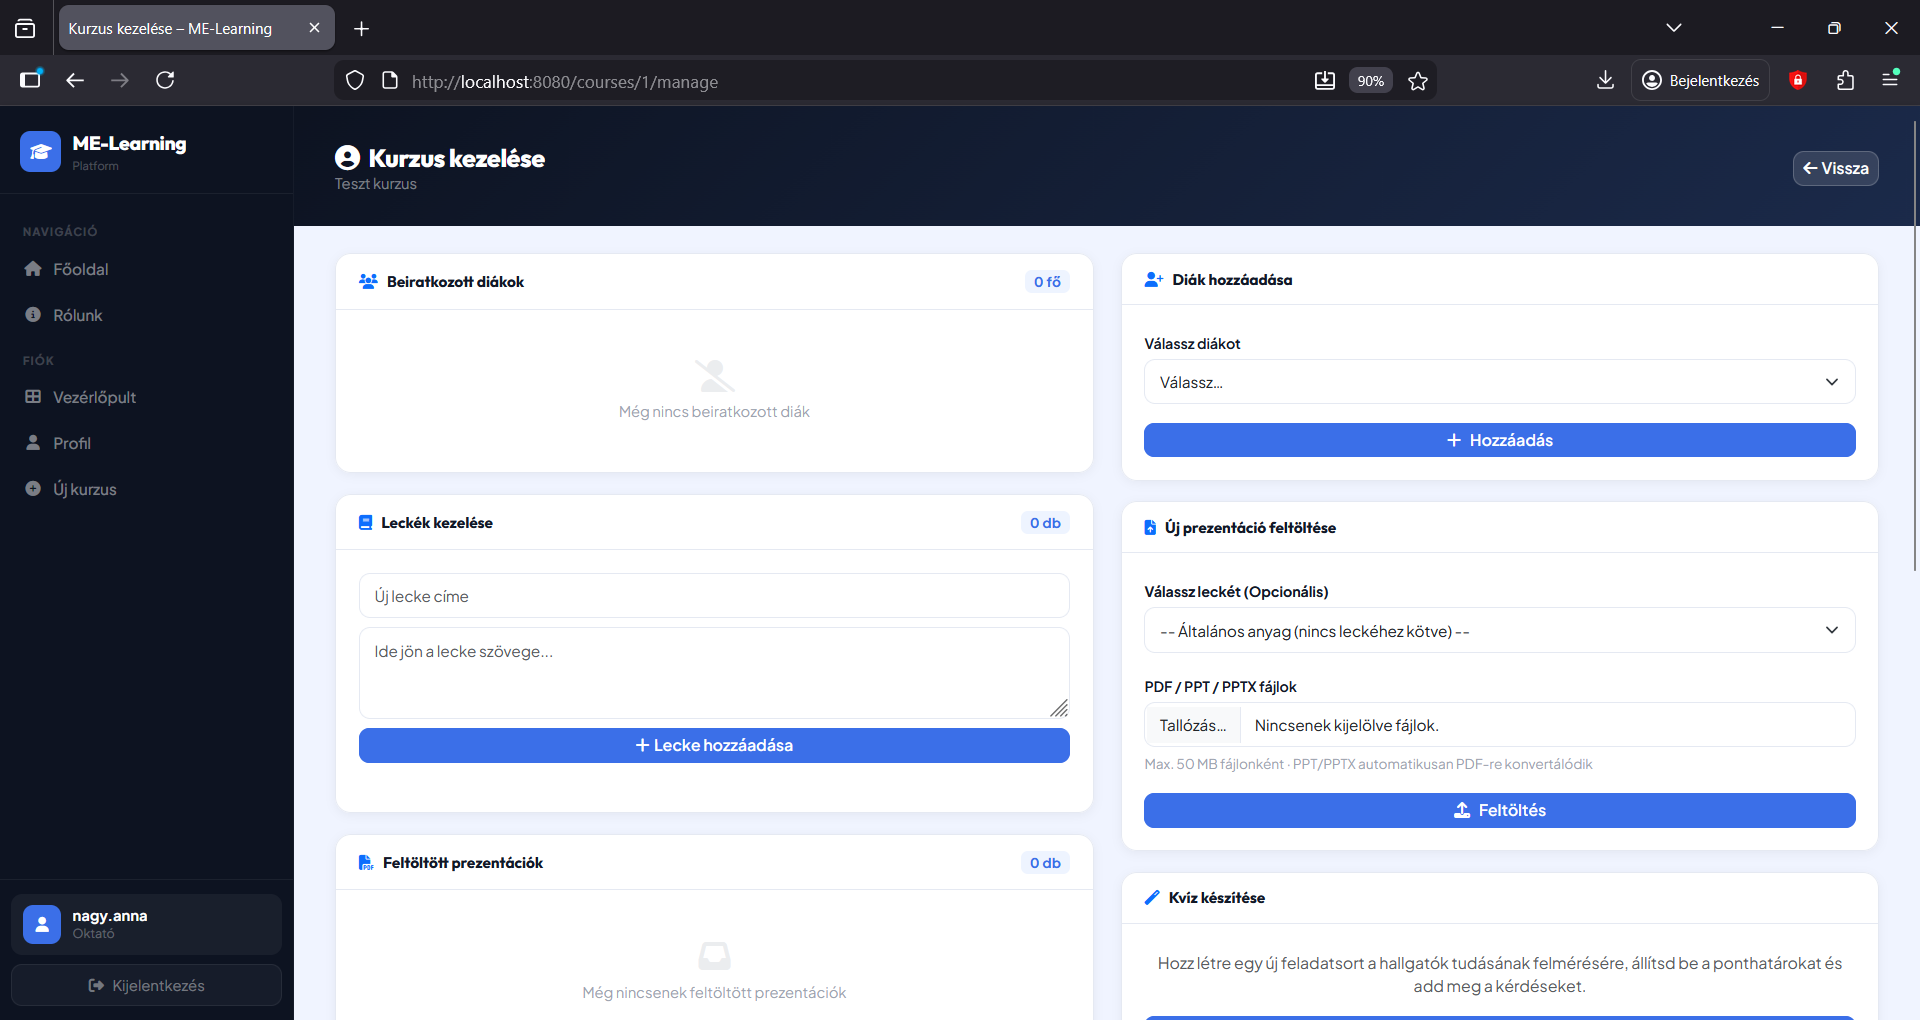
\includegraphics[width=1\textwidth]{images/Kurzus_kezelese.png}
    \caption{Kurzus kezelési oldal}
    \label{fig:Kurzus_kezelese}
\end{figure}

\begin{java}[caption={Kurzuslétrehozás},label=java:createcourse]
@PostMapping("/create")
public String createCourse(
        @Valid @ModelAttribute("course") Course course,
        Authentication auth,
        RedirectAttributes redirectAttributes) {

    Optional<User> instructorOpt = getCurrentUser(auth);

    try {
        course.setInstructor(instructorOpt.get());
        courseService.saveCourse(course);
        redirectAttributes.addFlashAttribute("success",
                "Kurzus sikeresen létrehozva!");
        return "redirect:/courses";
    } catch (Exception e) {
        redirectAttributes.addFlashAttribute("error",
                "Hiba történt a kurzus mentése során: "
                + e.getMessage());
        return "redirect:/courses/create";
    }
}
\end{java}

\subsection{Lecke létrehozása}

A lecke létrehozása a \texttt{POST /lessons/create} végponton keresztül történik. A kontroller a kérésben érkező \texttt{courseId} paraméter alapján azonosítja a szülő kurzust, beállítja a kapcsolatot a lecke és a kurzus között, majd elmenti az adatbázisba. A lecke létrehozásakor az oktató megadja a lecke címét, szöveges tartalmát és létrehozási sorrendben az indexét (\texttt{orderIndex}), amely meghatározza, hogy a lecke milyen sorrendben jelenik meg a kurzus oldalán. Sikeres mentés után a kontroller visszairányítja az oktatót a kurzus kezelőfelületére, ahol az újonnan létrehozott lecke azonnal megjelenik, és prezentációk is csatolhatók hozzá.

\begin{java}[caption={LessonController — lecke létrehozása},label=java:lessoncontroller]
@Controller
@RequestMapping("/lessons")
public class LessonController {

    @Autowired private LessonService  lessonService;
    @Autowired private CourseService  courseService;

    @PostMapping("/create")
    public String createLesson(@RequestParam Long courseId,
                                @ModelAttribute Lesson lesson) {
        Course course = courseService.getCourseById(courseId)
                .orElseThrow(() -> new IllegalArgumentException(
                        "Érvénytelen kurzus azonosító: " + courseId));
        lesson.setCourse(course);
        lessonService.save(lesson);
        return "redirect:/courses/" + courseId + "/manage";
    }
}
\end{java}

\subsection{Kurzusnézet leckékkel}

A \texttt{CourseController} kurzus-megtekintési végpontja a leckéket is betölti a modellbe, hogy a hallgatók a kurzus oldalán lecke-szinten is böngészhessenek.

\begin{figure}[h!]
    \centering
    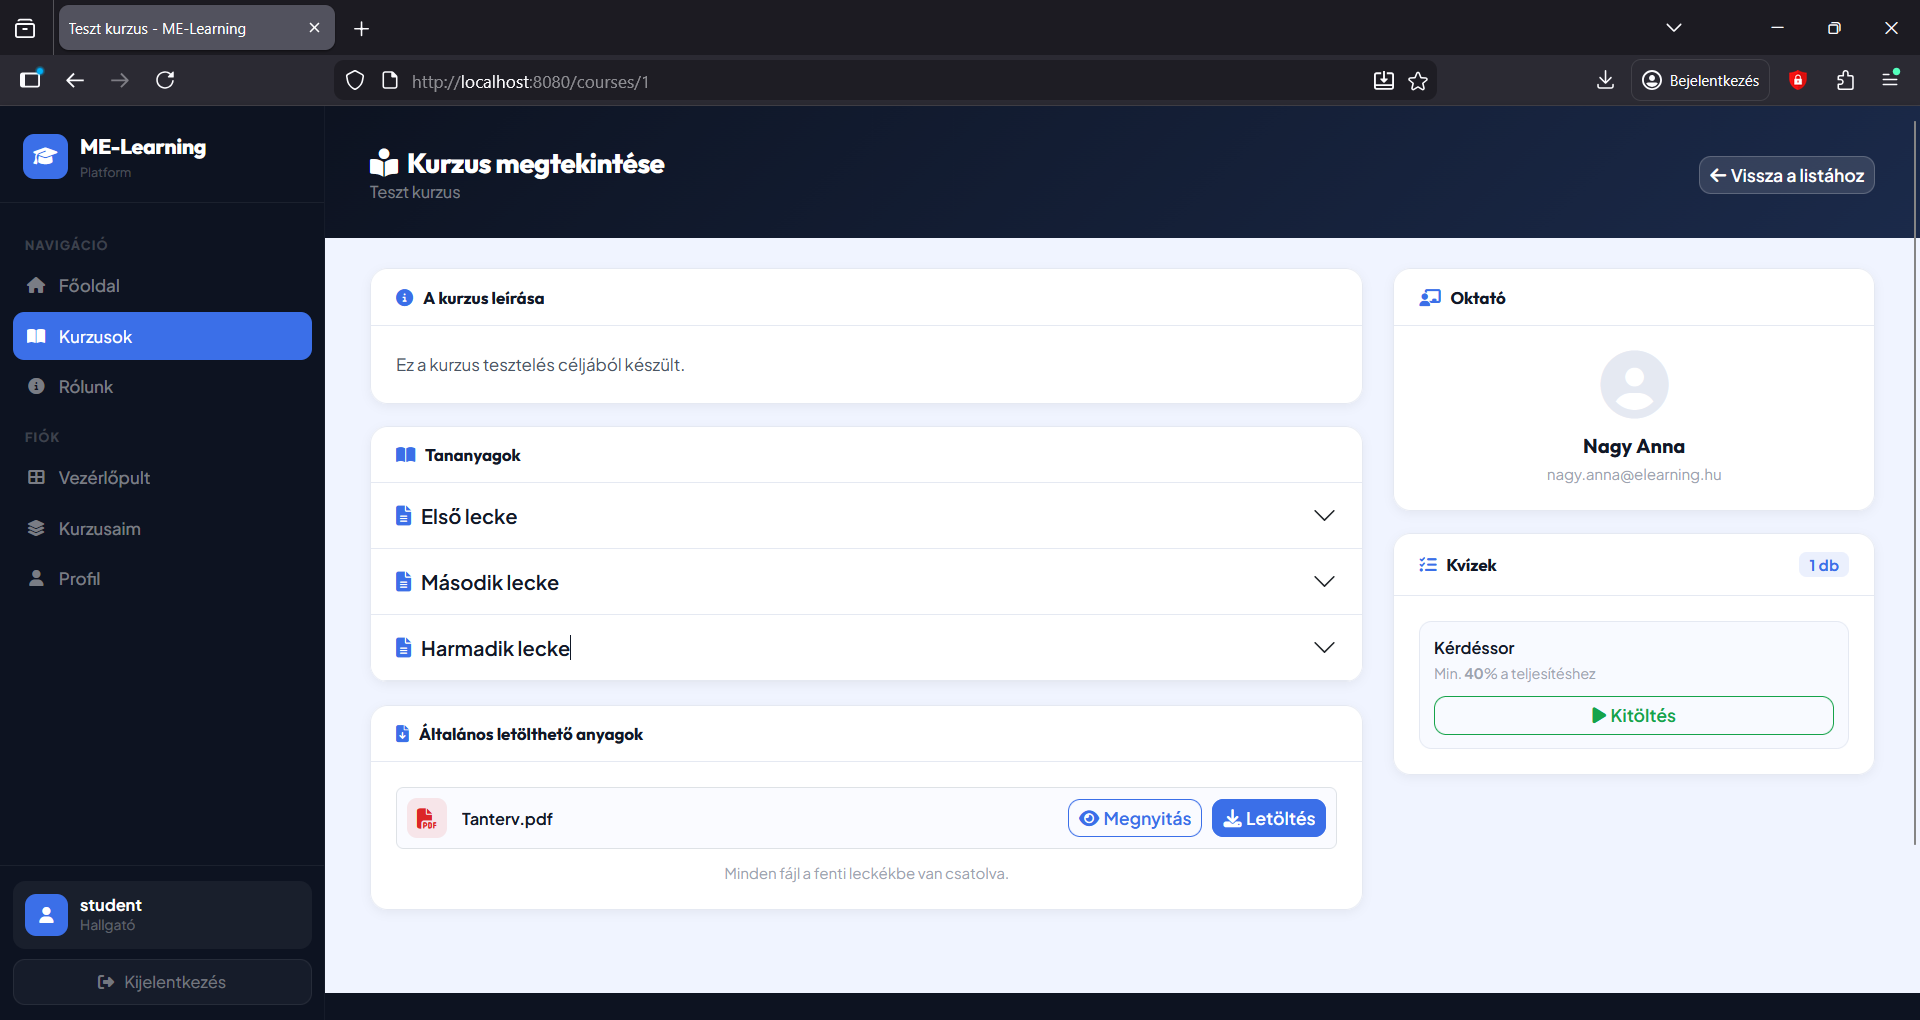
\includegraphics[width=1\textwidth]{images/Hallgatoi_nezet.png}
    \caption{Diákok nézete a beíratkozott kurzusra}
    \label{fig:Hallgatoi_nezet}
\end{figure}

\begin{java}[caption={Kurzusnézet — leckék betöltése a modellbe},label=java:viewcourse]
@GetMapping("/{id}")
public String viewCourse(@PathVariable Long id,
                          Model model, Authentication auth) {
    // ... jogosultság- és átirányítás-logika ...

    model.addAttribute("course",    courseObj);
    model.addAttribute("presentations",
            presentationService.getPresentationsByCourse(courseObj));
    model.addAttribute("quizzes",
            quizService.getQuizzesByCourse(courseObj));
    model.addAttribute("lessons",
            lessonService.findByCourseId(courseObj.getId()));

    return "courses/view";
}
\end{java}

A kurzusnézeten az admin és a saját kurzusát megtekintő oktató automatikusan a kezelőfelületre (\texttt{manage}) kerül átirányításra. A privát kurzust csak az oktató és a beiratkozott hallgatók láthatják.

\subsection{Prezentáció-feltöltés leckéhez rendeléssel és duplikáció-szűréssel}

A \texttt{POST /courses/\{id\}/add-presentations} végpont két fontos funkcióval bővült: az opcionális \texttt{lessonId} paraméter lehetővé teszi, hogy a feltöltött fájl egy konkrét leckéhez is hozzárendelődjön; a duplikáció-ellenőrzés pedig megakadályozza, hogy azonos nevű fájlt kétszer töltsön fel az oktató.

\begin{java}[caption={Prezentáció-feltöltés duplikáció-szűréssel és leckéhez rendeléssel},label=java:addpresent]
@PostMapping("/{id}/add-presentations")
public String addPresentations(
        @PathVariable Long id,
        @RequestParam("newPresentations") MultipartFile[] files,
        @RequestParam(required = false) Long lessonId,
        Authentication auth,
        RedirectAttributes redirectAttributes) {

    // ... jogosultság-ellenőrzés ...

    Lesson selectedLesson = null;
    if (lessonId != null) {
        selectedLesson = lessonService.findById(lessonId).orElse(null);
    }

    List<Presentation> existing =
            presentationService.getPresentationsByCourse(course);
    List<String> existingNames =
            existing.stream().map(Presentation::getFileName).toList();

    int order = existing.size() + 1;
    int addedCount = 0, skippedCount = 0;

    for (MultipartFile file : files) {
        if (!file.isEmpty()) {
            String orig  = file.getOriginalFilename();
            String lower = orig != null ? orig.toLowerCase() : "";
            if (lower.endsWith(".pdf") || lower.endsWith(".ppt")
                    || lower.endsWith(".pptx")) {

                String targetName = orig;
                if (lower.endsWith(".ppt") || lower.endsWith(".pptx"))
                    targetName = orig.substring(0,
                            orig.lastIndexOf('.')) + ".pdf";

                if (existingNames.contains(targetName)) {
                    skippedCount++;
                    continue;
                }

                presentationService.processAndSavePresentation(
                        file, course, selectedLesson, order++);
                addedCount++;
            }
        }
    }
    // ... visszajelző flash üzenetek ...
    return "redirect:/courses/" + id + "/manage";
}
\end{java}

A visszajelzés háromféle lehet: ha minden fájl kihagyásra kerül (már létezik), ha csak egy részük kerül feltöltésre, vagy ha mindegyik sikeresen feltöltött. Ez a részletes visszajelzés segít az oktatónak átlátni, mi történt a feltöltés során.

% ============================================================
%  4.10  Prezentáció-feldolgozás megvalósítása
% ============================================================

\section{Prezentáció-feldolgozás megvalósítása}

\subsection{A PresentationService}

A \texttt{PresentationService} feladata a feltöltött prezentációs fájlok feldolgozása és adatbázisba mentése. A \texttt{processAndSavePresentation()} metódus a feltöltött fájl kiterjesztése alapján dönt a feldolgozás módjáról: PDF fájl esetén a bájttömb közvetlenül mentésre kerül, míg \texttt{.ppt} és \texttt{.pptx} formátum esetén a metódus először PDF-fé konvertálja a fájlt, majd az így kapott bájttömböt menti el. A prezentáció egy kurzushoz kötelezően, egy leckéhez opcionálisan kapcsolódik — utóbbi \texttt{null} értékű is lehet, ha az oktató nem rendeli konkrét leckéhez a feltöltött anyagot.

\begin{java}[caption={A prezentáció-feldolgozó metódus},label=java:presentservice]
public Presentation processAndSavePresentation(
        MultipartFile file, Course course,
        Lesson lesson, Integer orderIndex) throws Exception {
    String fileName    = file.getOriginalFilename();
    byte[] fileData    = file.getBytes();
    String contentType = file.getContentType();

    if (fileName != null) {
        String lower = fileName.toLowerCase();
        if (lower.endsWith(".pptx") || lower.endsWith(".ppt")) {
            boolean isPptx = lower.endsWith(".pptx");
            fileData    = convertPptToPdfBytes(fileData, isPptx);
            fileName    = fileName.substring(0,
                            fileName.lastIndexOf('.')) + ".pdf";
            contentType = "application/pdf";
        }
    }

    Presentation p = new Presentation(
            fileName, fileData, contentType, course, lesson, orderIndex);
    return presentationRepository.save(p);
}
\end{java}

\subsection{PowerPoint–PDF konverzió}

A konverzió az Apache POI és az Apache PDFBox együttes alkalmazásával valósul meg. Az Apache POI két modulja eltérő formátumokat kezel: a \texttt{XMLSlideShow} osztály a modern \texttt{.pptx} (OOXML), a \texttt{HSLFSlideShow} osztály pedig a régebbi bináris \texttt{.ppt} formátumot dolgozza fel. A konverzió során a diák listáján végigiterálva minden egyes dia egy \texttt{BufferedImage}-re kerül renderelésre, amelyet az Apache PDFBox PDF-oldalként rögzít.

\begin{java}[caption={Dia renderelés és PDF-összeállítás},label=java:pptconvert]
private byte[] convertPptToPdfBytes(byte[] pptBytes, boolean isPptx)
        throws Exception {
    try (PDDocument pdfDocument = new PDDocument();
         ByteArrayInputStream  bais = new ByteArrayInputStream(pptBytes);
         ByteArrayOutputStream baos = new ByteArrayOutputStream()) {

        Dimension pgsize;
        List<?> slides;
        if (isPptx) {
            XMLSlideShow ppt = new XMLSlideShow(bais);
            pgsize = ppt.getPageSize();
            slides = ppt.getSlides();
        } else {
            HSLFSlideShow ppt = new HSLFSlideShow(bais);
            pgsize = ppt.getPageSize();
            slides = ppt.getSlides();
        }

        int scale = 3;
        int width  = (int)(pgsize.width  * scale);
        int height = (int)(pgsize.height * scale);

        for (Object slideObj : slides) {
            BufferedImage img = new BufferedImage(
                    width, height, BufferedImage.TYPE_INT_RGB);
            Graphics2D g = img.createGraphics();

            g.setRenderingHint(RenderingHints.KEY_ANTIALIASING,
                               RenderingHints.VALUE_ANTIALIAS_ON);
            g.setRenderingHint(RenderingHints.KEY_RENDERING,
                               RenderingHints.VALUE_RENDER_QUALITY);
            g.setRenderingHint(RenderingHints.KEY_INTERPOLATION,
                               RenderingHints.VALUE_INTERPOLATION_BICUBIC);
            g.setRenderingHint(RenderingHints.KEY_TEXT_ANTIALIASING,
                               RenderingHints.VALUE_TEXT_ANTIALIAS_ON);

            g.setPaint(Color.white);
            g.fill(new Rectangle2D.Float(0, 0, width, height));
            g.scale(scale, scale);

            if (isPptx) ((XSLFSlide) slideObj).draw(g);
            else        ((HSLFSlide) slideObj).draw(g);

            PDPage page = new PDPage(
                    new PDRectangle(pgsize.width, pgsize.height));
            pdfDocument.addPage(page);

            PDImageXObject pdImage =
                    JPEGFactory.createFromImage(pdfDocument, img, 0.90f);

            try (PDPageContentStream cs =
                         new PDPageContentStream(pdfDocument, page)) {
                cs.drawImage(pdImage, 0, 0, pgsize.width, pgsize.height);
            }
        }

        pdfDocument.save(baos);
        return baos.toByteArray();
    }
}
\end{java}

A képek 3-szoros skálán készülnek, ami azt jelenti, hogy az eredeti dia koordinátarendszeréhez képest háromszor akkora felbontású \texttt{BufferedImage} jön létre. A \texttt{Graphics2D} kontextust a \texttt{g.scale(scale, scale)} hívással skálázzuk, hogy a POI renderelője az eredeti koordinátarendszerben dolgozzon. A kész képet JPEG formátumban, 90\%-os minőséggel adjuk hozzá a PDFBox dokumentumhoz, miközben a PDF-oldal mérete az eredeti diával megegyező marad. Ez biztosítja, hogy a böngésző éles, jól olvasható képet jelenítsen meg.

\subsection{Prezentáció streamelése}

A \texttt{PresentationController} a tárolt PDF bájttömböt \texttt{ResponseEntity<byte[]>} formában streameli a böngésző felé. A \texttt{@Transactional} annotáció megakadályozza a \texttt{LazyInitializationException} hibát a lusta betöltésű \texttt{lesson} kapcsolat hozzáférésekor. A hozzáférés-ellenőrzés figyelembe veszi a kurzus láthatóságát is: nyilvános kurzus esetén bármely bejelentkezett felhasználó megtekintheti a prezentációt beiratkozás nélkül is, privát kurzusnál azonban csak az oktató és a beiratkozott hallgatók férhetnek hozzá.

\begin{java}[caption={PDF tartalom streamelése és hozzáférés-ellenőrzés},label=java:presentaccess]
@Controller
@Transactional
public class PresentationController {

    private boolean hasAccessToPresentation(
            Presentation presentation, Authentication auth) {
        if (auth == null) return false;
        Optional<User> userOpt =
                userService.getUserByUsername(auth.getName());
        if (userOpt.isEmpty()) return false;

        User   user   = userOpt.get();
        Course course = presentation.getCourse();

        if (user.getRole() == Role.ADMIN) return true;

        if (course.getInstructor() != null
                && course.getInstructor().getId().equals(user.getId()))
            return true;

        if (Boolean.TRUE.equals(course.getIsPublic())) return true;

        return course.getEnrolledUsers().contains(user);
    }
}
\end{java}

A streamelési végpont \texttt{ContentDisposition.inline()} fejlécet állít be, amely a böngészőt a beépített PDF-megjelenítő használatára ösztönzi letöltés helyett. Ha a fájl bájttömb üres vagy hiányzik, a végpont \texttt{404 Not Found} választ ad vissza.

% ============================================================
%  4.11  Kvízrendszer megvalósítása
% ============================================================
\section{Kvízrendszer megvalósítása}

\subsection{Kvíz kitöltési és kiértékelési logika}

A \texttt{GET /courses/\{courseId\}/quizzes/\{quizId\}/take} végpont induláskor ellenőrzi, hogy a hallgató korábban már kitöltötte-e a kvízt, és az egyszeri kitöltés be van-e kapcsolva. Ha igen, az előző eredmény kerül megjelenítésre.

A \texttt{POST /courses/\{courseId\}/quizzes/\{quizId\}/submit} végpont szerver oldalon értékeli ki az eredményt: a beküldött válaszokat (\texttt{question\_\{id\}} paraméterneveken) összehasonlítja a tárolt helyes válaszokkal, kiszámolja a százalékos teljesítményt, és a \texttt{Quiz.calculateGrade()} metódussal meghatározza az érdemjegyet.

\subsection{Ponthatár-módosítás visszamenőleges hatása}

A \texttt{POST /courses/\{courseId\}/quizzes/\{quizId\}/thresholds} végpont az új ponthatárok elmentése után az összes korábbi \texttt{QuizResult} osztályzatát újraszámítja, majd \texttt{saveAll()} hívással egyetlen tranzakcióban menti a változásokat.

\begin{java}[caption={Visszamenőleges osztályzat-újraszámítás ponthatár-módosítás után},label=java:threshold]
quiz.setExcellentThreshold(excellentThreshold);
quiz.setGoodThreshold(goodThreshold);
quiz.setAverageThreshold(averageThreshold);
quiz.setPassingThreshold(passingThreshold);
quiz.setAllowMultipleAttempts(allowMultipleAttempts);
quizService.saveQuiz(quiz);

List<QuizResult> results = quizResultRepository.findByQuiz(quiz);
for (QuizResult r : results) {
    r.setGrade(quiz.calculateGrade(r.getPercentage()));
}
quizResultRepository.saveAll(results);
\end{java}

% ============================================================
%  4.12  E-mail értesítési rendszer
% ============================================================
\section{E-mail értesítési rendszer}

Az \texttt{EmailService} öt HTML-alapú e-mail típust kezel: regisztrációs üdvözlőlevelet, jelszóváltoztatási értesítőt, felhasználónév-módosítási értesítőt, e-mail-változtatási értesítőt, és fióktörlési visszaigazolást. Az e-mail törzsek Java szövegtömbökkel (\textit{text blocks}) és \texttt{String.formatted()} behelyettesítéssel épülnek fel. Az e-mail küldési hiba szándékosan csak naplózásra kerül, és nem propagálódik, hogy SMTP-hiba ne akassza meg a felhasználói folyamatot.

% ============================================================
%  4.13  Nézetek és sablon-rendszer
% ============================================================
\section{Nézetek és sablon-rendszer}

\subsection{Sablon-struktúra}

A nézetek az \texttt{src/main/resources/templates/} könyvtárban helyezkednek el, funkcionális területenként alkönyvtárakba szervezve:

\begin{sloppypar}
\begin{itemize}
    \item Gyökérszintű sablonok: \texttt{index.html}, \texttt{login.html}, \texttt{register.html}, \texttt{profile.html}, \texttt{about.html}.
    \item \texttt{courses/}: \texttt{list.html}, \texttt{view.html}, \texttt{create.html}, \texttt{manage.html}, \texttt{viewer.html} (diavetítő), \texttt{take-quiz.html}, \texttt{quiz-result.html}, \texttt{quiz-results.html}, \texttt{quiz-thresholds.html}, \texttt{create-quiz.html}.
    \item \texttt{dashboard/}: \texttt{admin.html}, \texttt{instructor.html}, \texttt{student.html}.
    \item \texttt{presentation/}: \texttt{viewer.html}.
    \item \texttt{fragments/}: \texttt{sidebar.html}.
    \item \texttt{error/}: \texttt{404.html}, \texttt{error.html}.
\end{itemize}
\end{sloppypar}

\subsection{Mobiloptimalizálás és reszponzív nézetek}

Az optimalizálás során az összes sablon reszponzív megjelenítésre lett felkészítve. A Bootstrap keretrendszer rácsrendszere (\texttt{col-md-*}, \texttt{col-sm-*} osztályok) biztosítja, hogy a tartalom asztali, tabletes és mobilos képernyőn egyaránt olvasható elrendezést vegyen fel. A navigációs sáv mobilon összecsukható hamburger-menüként jelenik meg.

A kurzuslista kártya-alapú elrendezést (\texttt{card}) alkalmaz, amelyek mobilon teljes szélességűek, asztali nézetben pedig többoszlopos rácsban helyezkednek el. A kvízkitöltő és az eredményoldal gombjainak mérete és tapintható területe is mobil-barát értékekre lett beállítva.

\subsection{Thymeleaf–Spring Security integráció}

A \texttt{thymeleaf-extras-springsecurity6} függőség aktiválja a \texttt{sec:} névteret, amely HTML-szinten teszi lehetővé a szerepkörfüggő megjelenítést:

\begin{java}[caption={Szerepkörfüggő megjelenítés Thymeleaf sablonban},label=java:thymeauth]
<div sec:authorize="hasRole('INSTRUCTOR')">
    <a th:href="@{/courses/create}">Kurzus létrehozása</a>
</div>

<span sec:authorize="isAuthenticated()"
      th:text="${#authentication.name}">
    Felhasználónév
</span>
\end{java}

Ez a megközelítés kizárólag megjelenítési szintű elrejtést valósít meg; a tényleges hozzáférés-védelmet minden esetben a Spring Security szűrőlánc és a service-szintű ellenőrzés biztosítja.

\subsection{Statikus erőforrások}

A \texttt{static/css/} könyvtár két stíluslapot tartalmaz: a \texttt{main.css} az összes hitelesített oldal egységes vizuális stílusát határozza meg, a \texttt{landing.css} pedig a nyilvánosan elérhető főoldal egyedi megjelenését — ez megakadályozza, hogy a nyilvános oldal stílusai felülírják az alkalmazás belső stílusait.
